The test were conducted using a gateway connected to 4 nodes. The nodes were place each on a shelf in order to see if the height of the shelf might replicate a tall building. The nodes needed to be mounted securely, otherwise the data would have been courupted. This applies to the real world, where the nodes will need a sturdy mounting place to properly sence any vibrations in the structure of the building.


We have conducted 3 tests by seting the shake table at different voltages and the same ammount of vibration time of 3 seconds.
\begin{itemize}

\item Test at 2v. This test will demonstrate that even when the table is barely vibrating in order to simulate a small eartquake, the nodes are capable of detecting it.
\item Test at 4v. This is a more stronger test.
\item Test at 7v. This generates powerfull vibrations which help us see if the limit of +/-2G set on the nodes can be reached.
\end{itemize}

\begin{figure}[ht] \centering
  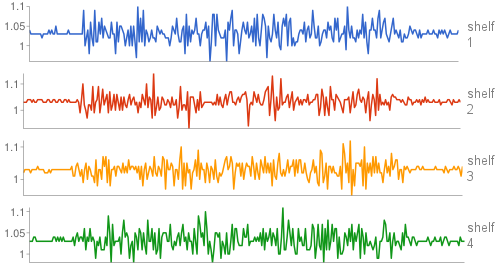
\includegraphics[width=0.5\textwidth]{img/2v.png}
  \caption{Results for the shake table at 2V}
  \label{fig:2v}
\end{figure}

\begin{figure}[ht] \centering
  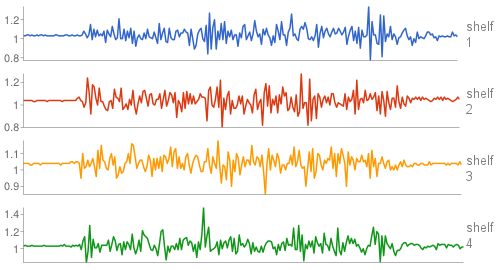
\includegraphics[width=0.5\textwidth]{img/4v.png}
  \caption{Results for the shake table at 4V}
  \label{fig:4v}
\end{figure}

\begin{figure}[ht] \centering
  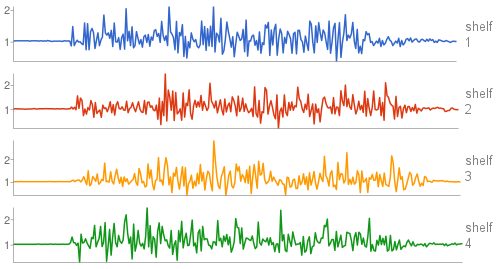
\includegraphics[width=0.5\textwidth]{img/7v.png}
  \caption{Results for the shake table at 7V}
  \label{fig:7v}
\end{figure}

As it can be seen in figure~\ref{fig:2v}, figure~\ref{fig:4v} and figure~\ref{fig:7v}, the value range when the table is still is around 1G with a diference of 0.04G. Any value that is higer or lower than that and is relatively periodical can be interepreted as an eartquake. 

The results prove that the experimental rig is responding similar to a tall building because the lower positioned nodes gather stronger values then the ones located on higher shelfs when the table is vibrating. In the end of the simulation, when the table is not shaken and it is naturaly vibrating due to previous forces, the higher positioned nodes continue to detect vibrations, as it should have happened in the case of a real building.
